\chapter{Projektplanung}
\begin{figure}[H]
  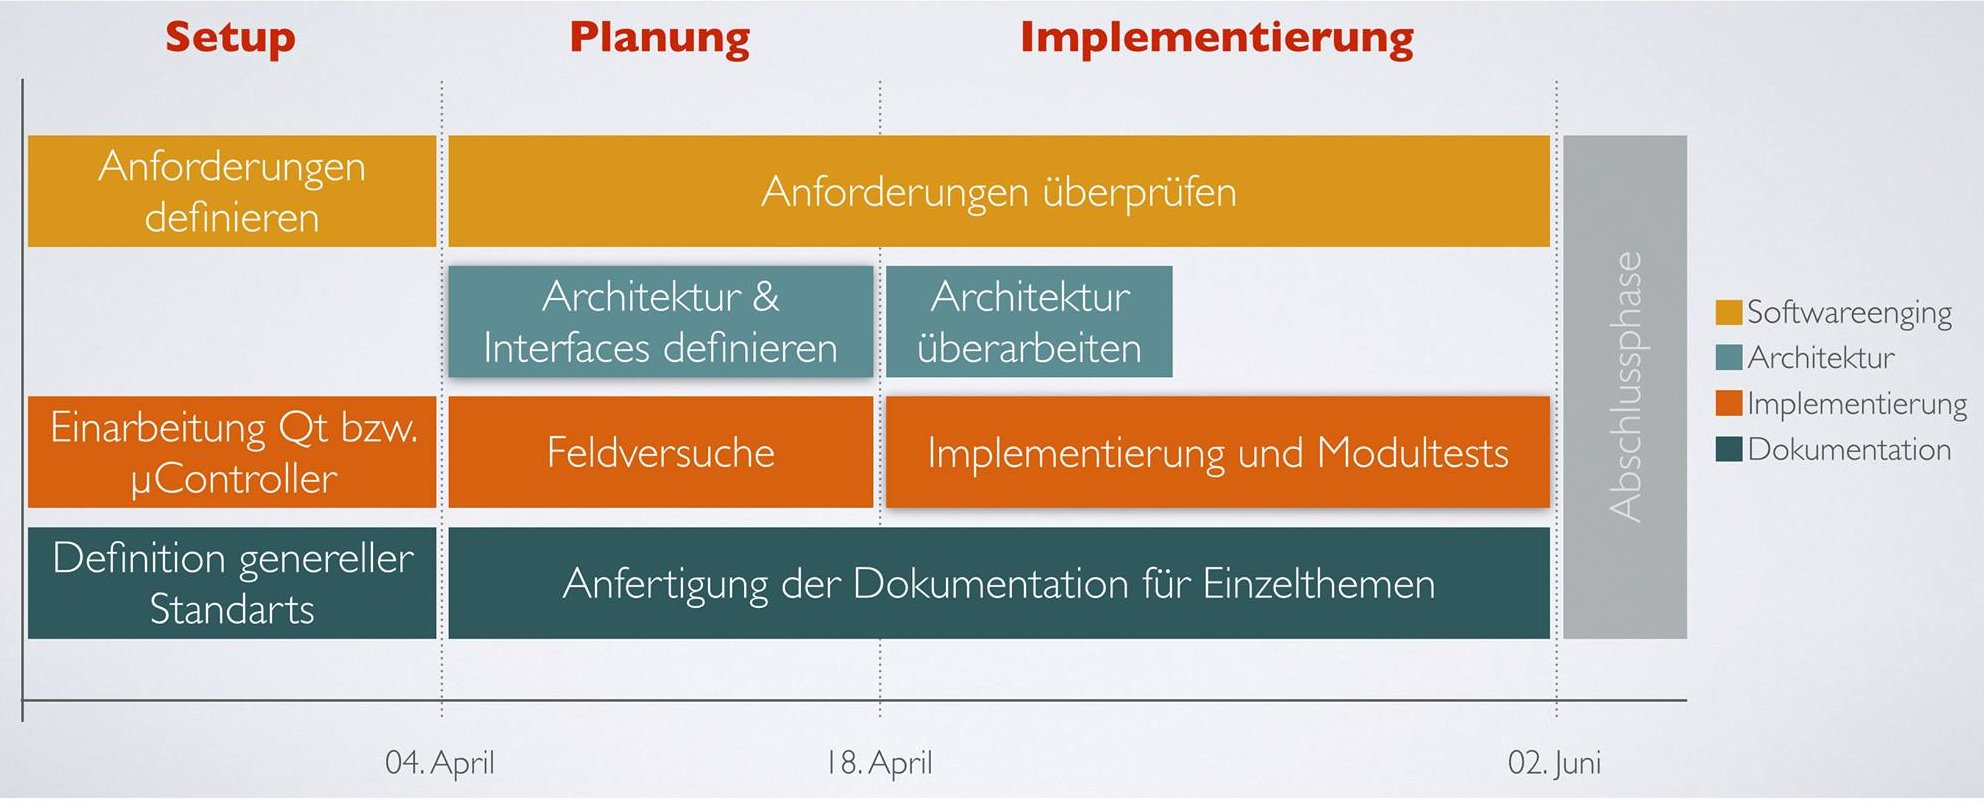
\includegraphics[width=12cm]{content/pictures/Zeitplan.jpg}
  \caption{Zeitplan}
  \label{anh: Zeitplan}
\end{figure}
Bei der Projektplanung wurde zu Beginn des Semesterprojektes ein Zeitplan erstellt, mit genauen Terminen und 
Meilensteinen, an welchen sich gehalten wurde. Zudem wurden zu Beginn Anforderungen definiert (siehe Anhang), 
welche bis zum Ende des Prjektes abgearbeitet wurden.
Anbei eine tabellarische Auflistung unseres zeitlichen Verlaufs:

\section{Zeitlicher Ablauf}

%Issue #11 Beachten
\begin{table}[H]
\begin{tabular}{ll}
26.03.2014 & Erstes Einlesen in die Problematik \\
& Postenverteilung\\
& Festlegen von Standards (Git, Felix,\ldots) \\
& Erstellung des Zeitplans \\
02.04.2014 & Board in Betrieb genommen\\
& GitHub eingerichtet\\ 
&Dokumentation begonnen\\ 
& Problematik von Speicher des ATMega32\\
& Ausweichen auf ATMega644p vorgeschlagen \\
\textbf{Meilenstein} 04.04.2014 & Setup-Phase abgeschlossen \\
& Anforderungen sind definiert\\
& es wurde sich in die 
Themengebiete eingelesen\\
& Standards wurden definiert und umgesetzt\\
\textbf{Meilenstein} 18.04.2014 & Planungs-Phase abgeschlossen \\
& Archtitektur und Interfaces wurden definiert\\
& Feldversuche (Radig as Is läuft auf Board) abgeschlossen \\
& Doku wurde begonnen\\
30.04.2014 & Debugger erhalten\\
& ATmega644p in Betrieb genommen\\
& Implementierung an Webseite\\
& Weiterarbeit an Doku\\
07.05.2014 & Board: Pins schaltbar
\\
& Webseite: favorite.js fertig \\
14.05.2014 & Webseite: Übersichtseite fertig\\
& Seitenleiste verwendbar\\
& Pins setzen möglich\\
21.05.2014 & Webseite: Feinschliff\\ 
&Abänderung der Favoriten zu einer Liste aller Pins\\
& Pins zu Ein- und Ausgänge schaltbar \\
28.05.2014 & Webserver minimiert\\
& Skriptfunktionen hinterlegbar\\
& Favoriten in lokale Datenbank ausgelagert \\
\textbf{Meilenstein} 02.06.2014 & Implementierungsphase abgeschlossen \\
& Code-Freeze\\
bis 30.06.2014 & Code-Clean-Up\\
& Feinschliff Dokumentation\\
& Erstellen von Plaktaten\\
\end{tabular}
\end{table}


